\documentclass{article}
\usepackage[utf8]{inputenc}
\usepackage{amsmath,amsfonts,amssymb}
\usepackage{mathtools}
\DeclarePairedDelimiter{\ceil}{\lceil}{\rceil}
\usepackage{graphicx}
\usepackage{float}
\usepackage{listings}
\usepackage{bbm}
\usepackage{indentfirst}
\usepackage{blindtext}
\usepackage{titlesec}
\usepackage[utf8]{inputenc}
\usepackage{listings}
\usepackage{braket}
\usepackage{tikz}
\usetikzlibrary{quantikz}
\usepackage{algorithm}
\usepackage{algorithmic}
\usepackage[english]{babel}
\usepackage{biblatex}
\usepackage{xcolor}
\usepackage{MnSymbol,wasysym}
\usepackage{hyperref}
\usepackage{graphicx}

\addbibresource{finalproject.bib}

\title{Lab Project}
\author{Ronen Rojas}
\date{September 2021}


\begin{document}

\maketitle
\tableofcontents


\newpage
\section{Abstract} 

Main points
\begin{itemize}
	\item We've trained an LSTM model on precipitation in Godavari basin in India and also (CAMELS?)
	\item Static/ no static data of internal basins.
	\item Implemented integrated gradients on the LSTM.
	\item We've trained an CNN-LSTM model on spatial precipitation in Godavari basin in India
	\item Implemented integrated gradients on the CNN-LSTM 
	\item Implemented SHAP on the CNN-LSTM 
	\item Spatial and temporal visualization of the attributes.

\end{itemize}



\newpage
\section{Interpretability}

\subsection{What is Interpretability} 

In recent years machine learning models became the "go-to" solution for almost every task of estimation or prediction. It has Replaced the somewhat tedious task of trying to manually extract insights from the data.\\

It is definitely easier in a sense to let the computer "learn" from the data whatever it needs, all you need is a strong GPU and good clean data, once you've got all your ducks in a row you're good to go. The performance of these kind of models is uncanny and unprecedented (\cite{he2015deep}, \cite{DBLP:journals/corr/abs-1805-01890}, \cite{DBLP:journals/corr/abs-1905-01392}).\\

But with great power comes great responsibility, how do we explain a model prediction in a sensible manner. Most models are considered to be \textit{"black boxes"} and humanly incomprehensible. We are now interested more on "why" and less on "what" and most of the time a simple accuracy metric is not enough.\\

Interpretability tries to tackle this issue and tries to answer these lines of questions:
\begin{itemize}
	\item \textit{Why did the model made that prediction ?}	
	\item \textit{Do we have a human-friendly explanation for this prediction ?}	
	\item \textit{Can we visualize this explanation ? }	
\end{itemize}


According to \cite{molnar2019} we also need to formalize what is a good explanation, can we generalize it to a group of predictions instances ? is it model agnostic ?\\

In the next section we'll overview some of the main interpretability methods we've incorporated. \\

\newpage
\subsection{Historical overview} 

We have tried to divide it to 3 main groups:
\begin{enumerate}
	\item Gradient Visualizations
	\item Input driven insight
	\item Internal structural insights
\end{enumerate} 

\subsubsection{Saliency maps}

\subsubsection{Integrated gradients}

\subsubsection{Shapley values}


\newpage

\section{Models}
\subsection{Feed Forward Neural Network}

\subsubsection{Neural Network - Introduction}
\begin{itemize}
	\item $y = f_{W}(x), x \in \mathbb{R}^n, y \in \mathbb{R}^m$ 
	\item $W$ Learn-able parameters
	\item Data set $\{x_i, y_i \}_{i=1}^k$
	\item Loss function $L(f(x_i), y_i)$
	\item Gradient decent $W_t = W_{t-1} + \alpha \nabla_{W}L(x,y) $ 
\end{itemize}

\begin{figure}[H]\centering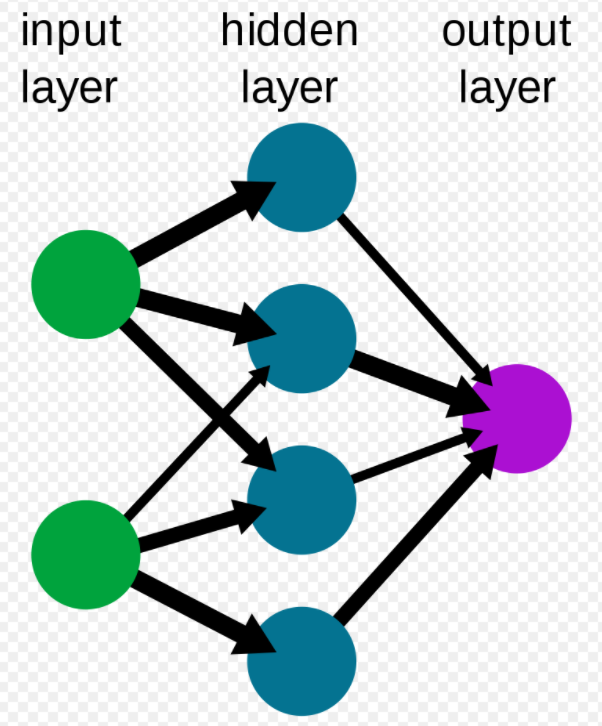
\includegraphics[width=6cm]{FFNN.png}\caption{Neural Network Architecture}\end{figure}

\newpage
\subsubsection{Neural Network - Function definitions}
\begin{itemize}
	\item Affine layer $y = Ax + b , x \in \mathbb{R}^n, b, y \in \mathbb{R}^m, A \in \mathbb{R}^{m \times n}$
	\item Activation point wise
	\begin{itemize}
		\item $\sigma_g(z) = \frac{1}{1+e^{-z}}$ - Sigmoid 
		\item $ReLU(z) = \max(0, z)$  - Rectified linear unit
	\end{itemize}	
\end{itemize}

\begin{figure}[H]\centering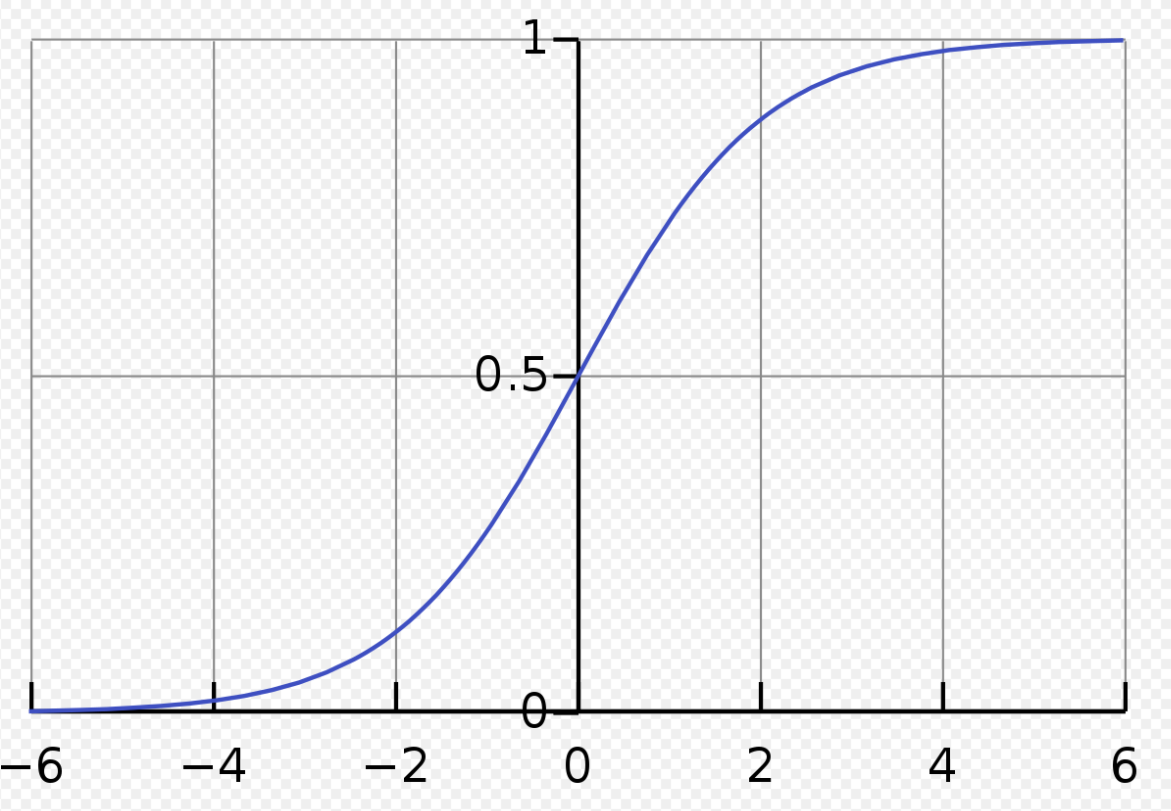
\includegraphics[width=6cm]{sigmoid.png}\caption{Sigmoid function}\end{figure}
\begin{figure}[H]\centering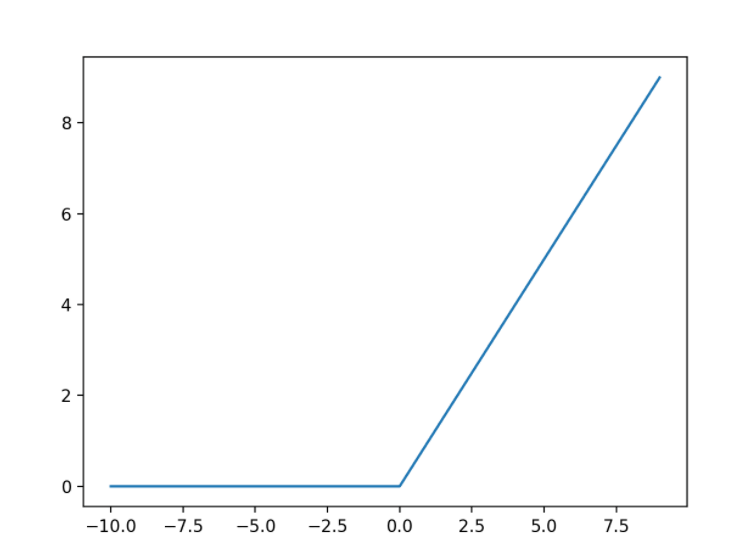
\includegraphics[width=6cm]{RELU.png}\caption{ReLU function}\end{figure}

\newpage
\subsubsection{Neural Network - Layering functions}

\begin{itemize}
	\item Dense: $y = \sigma(L), L = Ax+b$
	\item Expressiveness 
	\item Back propagation - $\frac{\partial y}{ \partial w} =  \frac{\partial y}{ \partial L} \cdot \frac{\partial L}{ \partial w}$
\end{itemize}


\subsubsection{Neural Network - Hyperbolic tangent  function}
$\sigma_h = \tanh(z) = \frac{e^z-e^{-z}}{e^z+e^{-z}}$
\begin{figure}[H]\centering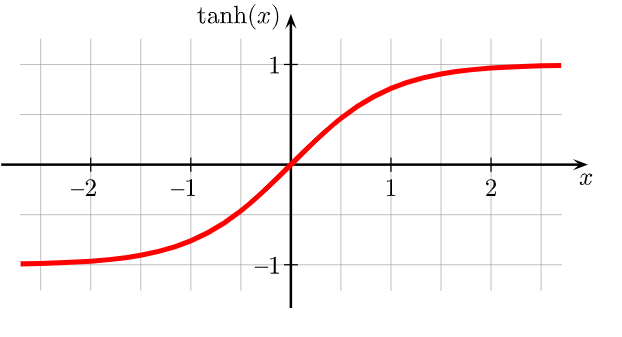
\includegraphics[width=6cm]{tanh.png}\caption{Hyperbolic tangent function}\end{figure}


\subsubsection{Neural Network - Problems}


\begin{itemize}
	\item Fixed size input
	\item No memory
\end{itemize}


\newpage
\subsection{RNN}

\subsubsection{RNN - Introduction}
\begin{itemize}
	\item Signals with timestamp (time series) - $\{x_t, y_t \}_{t=1}^k$
	\item Hidden state - $h_t = f_{W}(x_t, h_{t-1})$
	\item Same weights $W$ for each step
	\item Popular in Natural Language Processing (NLP)
\end{itemize}
\begin{figure}[H]\centering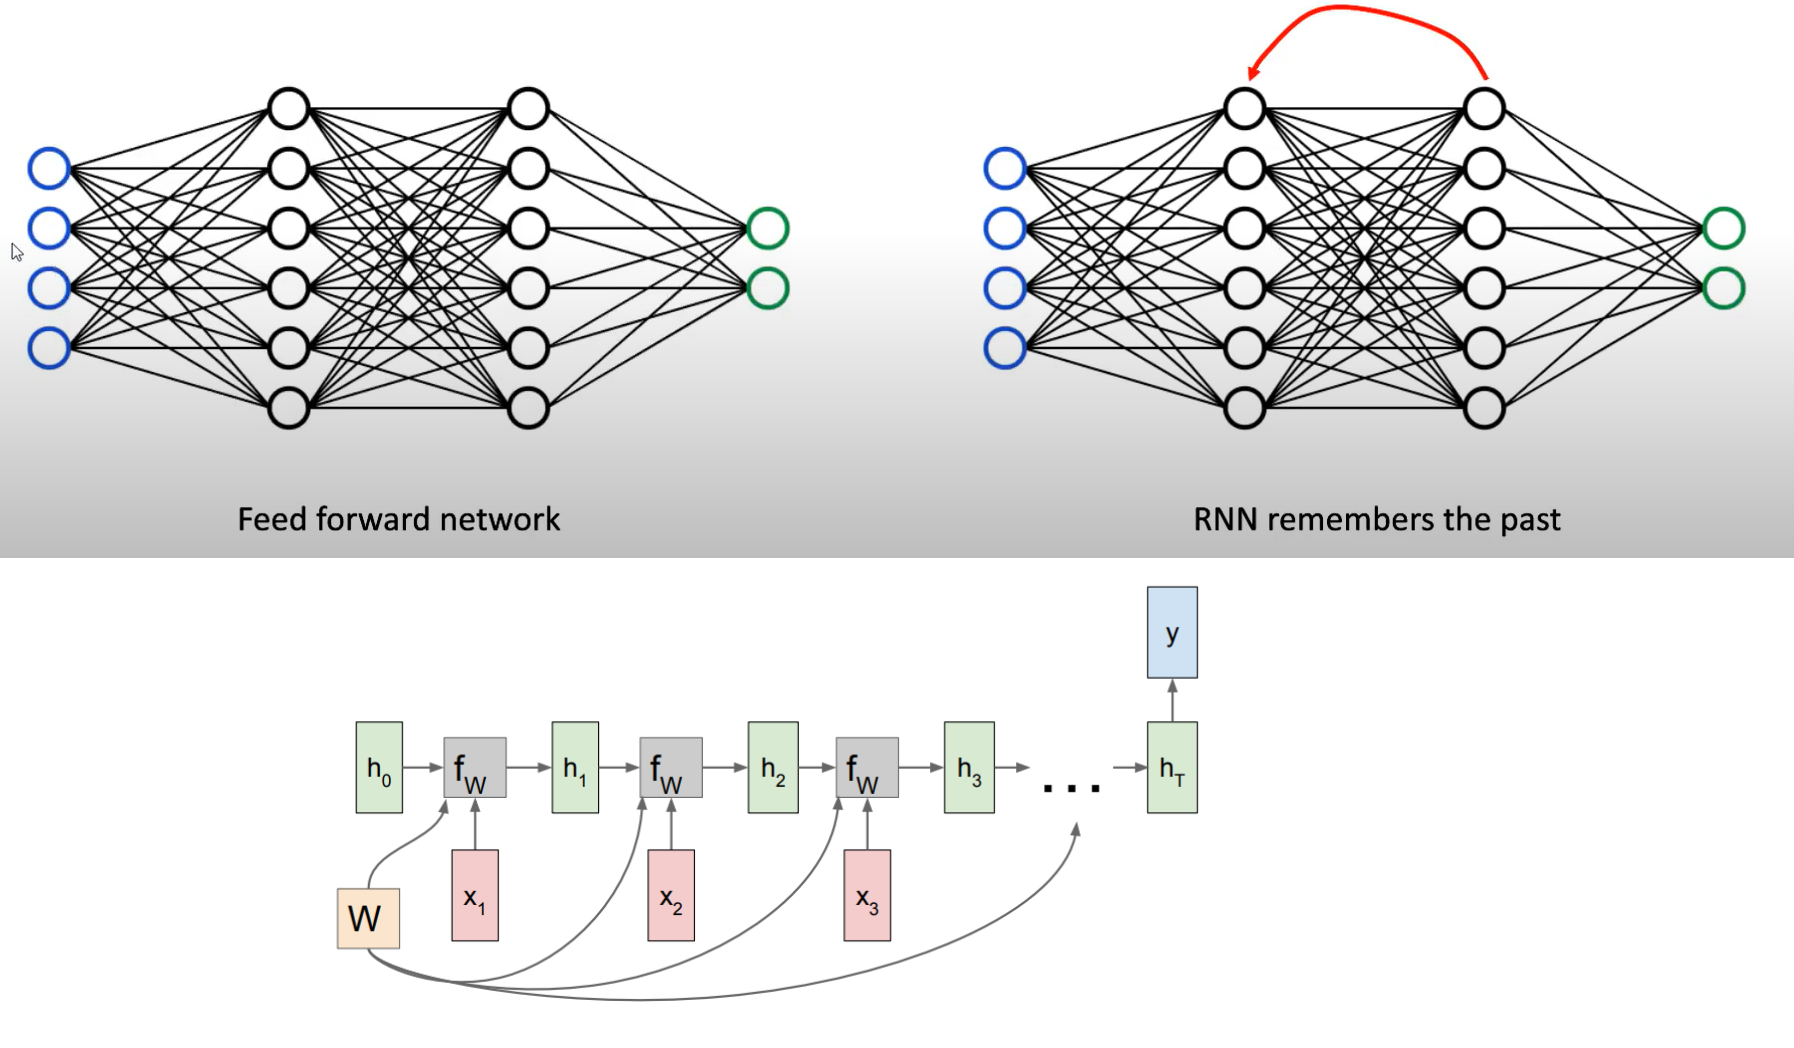
\includegraphics[width=10cm]{RNN.png}\caption{RNN}\end{figure}


\subsubsection{RNN - Simple example}

\begin{itemize}
	\item $h_t = \sigma_h \big(W_{hh} h_{t-1} +  W_{xh} x_{t} + b_h\big)$
	\item $y_t  = W_{hy} h_{t} +  b_y$
\end{itemize}

\subsubsection{RNN - Multi-Layer}
\begin{figure}[H]\centering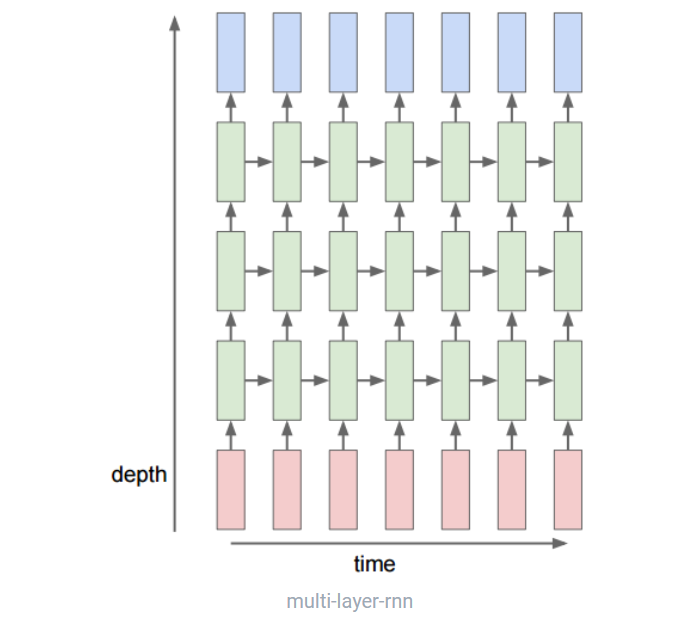
\includegraphics[width=10cm]{RNN_MULTI.png}\caption{RNN - MultiLayer}\end{figure}
\begin{align*}
h_t^{layer} = \sigma_h \bigg(W^{layer} \begin{pmatrix}
h_{t}^{layer-1} \\ h_{t-1}^{layer}
\end{pmatrix} \bigg)
\end{align*}


\subsubsection{RNN - Training }
Back propagation through time:
\begin{figure}[H]\centering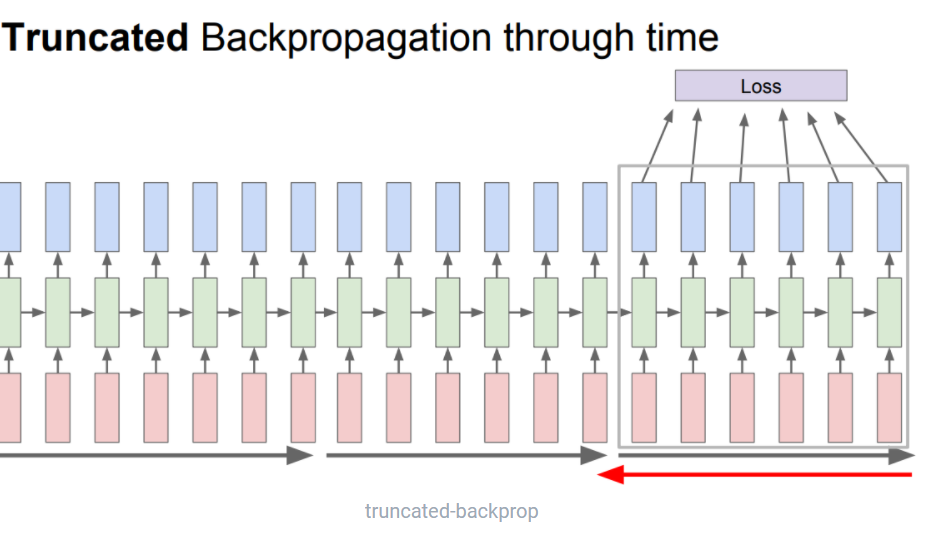
\includegraphics[width=10cm]{RNN_BACKPROP.png}\caption{RNN - back propagation}\end{figure}


\subsubsection{RNN - Problems}

Small example, scalars and no hidden states:
\begin{figure}[H]\centering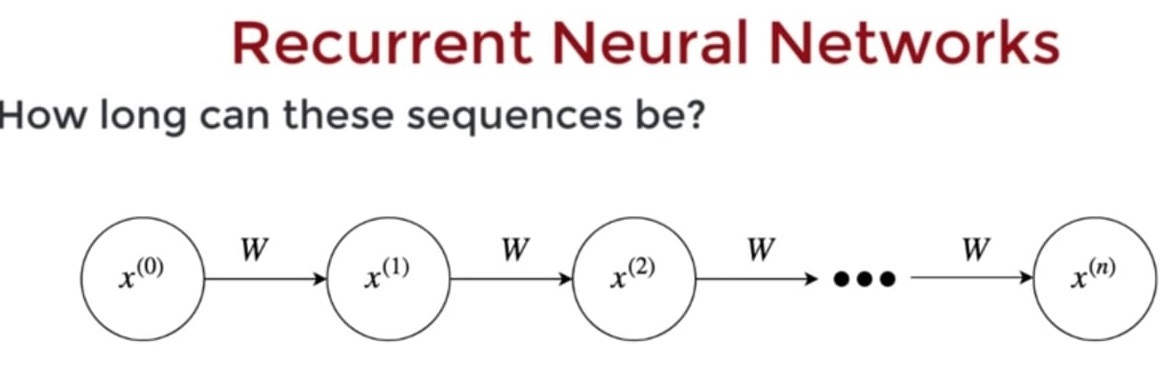
\includegraphics[width=10cm]{Explode.jpeg}\caption{RNN - Exploding vanishing gradients}\end{figure}

\begin{itemize}
	\item Exploding vanishing gradients
	\item $x^{(n)} = W^t x^{(0)}$
	\item 10 time steps.
\end{itemize}

\newpage
\subsection{LSTM}


\subsubsection{LSTM - Motivation}

LSTM (Long Short Term Memory) is a special kind of RNN,  designed to overcome the limitation of RNN
\begin{itemize}
	\item Gradient vanishing and exploding
	\item Complex training
	\item Difficulty to processes long sequences 
\end{itemize}

Remembering information for long periods of time is intrinsic to LSTM.

\subsubsection{LSTM - Principles}


\begin{figure}[H]\centering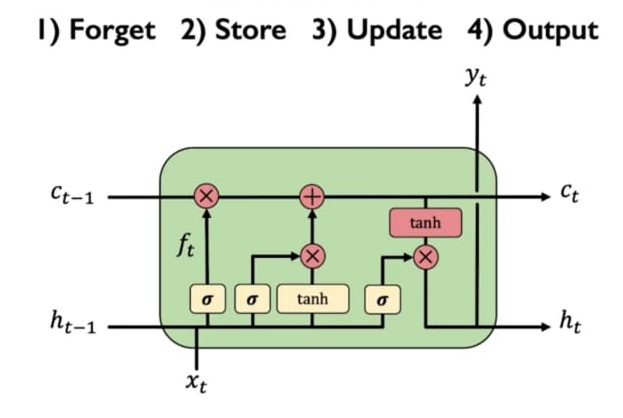
\includegraphics[width=7.5cm]{LSTM_MAIN.jpeg}\caption{LSTM - Scheme}\end{figure}

\begin{figure}[H]\centering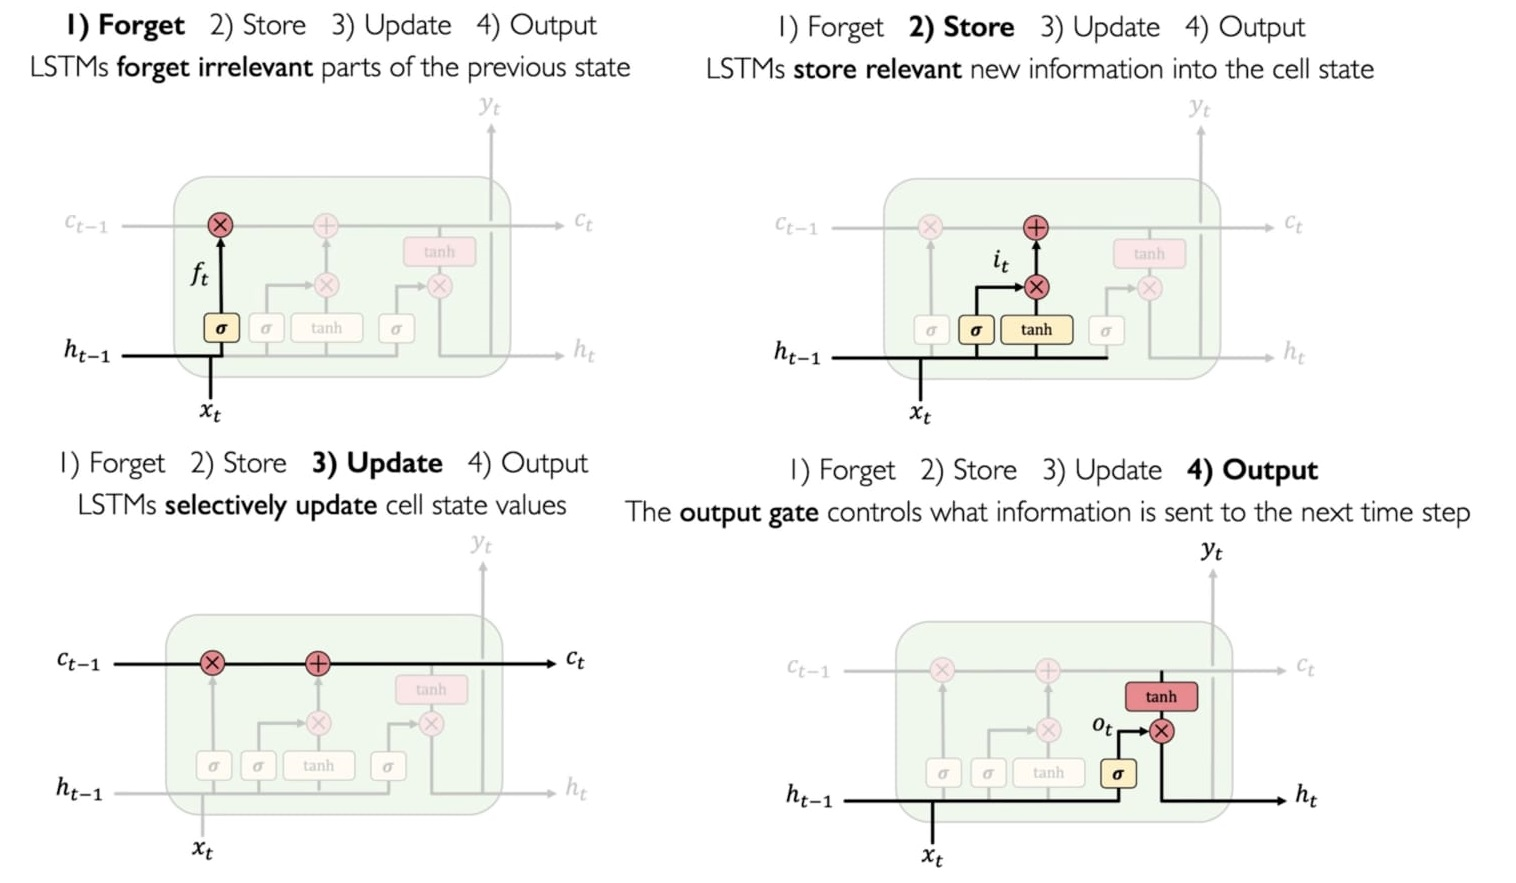
\includegraphics[width=14cm]{LSTM_SCHEME.jpeg}\caption{LSTM - Scheme}\end{figure}

\begin{itemize}
	\item Separate Cell state
	\item Gate to control flow of information:
	\begin{itemize}
		\item \textbf{Forget} - Gets rids of irrelevant information.
		\item \textbf{Store} - Relevant information from input
		\item \textbf{Update} - Selectively update cell state
		\item \textbf{Output}
	\end{itemize}
\end{itemize}


\begin{figure}[H]\centering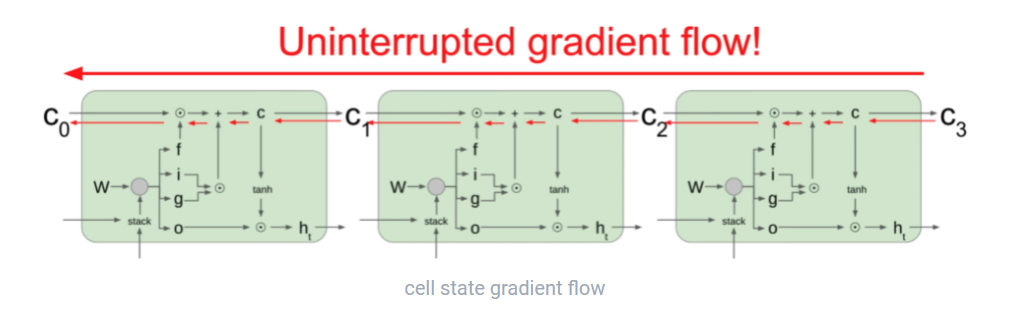
\includegraphics[width=10cm]{LSTM_GRADIENT_FLOW.png}\caption{LSTM - Gradient flow}\end{figure}


\subsubsection{LSTM- Formulation}
\begin{align*}
f_t &= \sigma_g(W_{f} x_t + U_{f} h_{t-1} + b_f) \\
i_t &= \sigma_g(W_{i} x_t + U_{i} h_{t-1} + b_i) \\
o_t &= \sigma_g(W_{o} x_t + U_{o} h_{t-1} + b_o) \\
\tilde{c}_t &= \sigma_c(W_{c} x_t + U_{c} h_{t-1} + b_c) \\
c_t &= f_t \circ c_{t-1} + i_t \circ \tilde{c}_t \\
h_t &= o_t \circ \sigma_h(c_t)
\end{align*}

where the initial values are $c_0 = 0$ and $h_0 = 0$ and the operator $\circ$ denotes the Hadamard product (element-wise product). 

\begin{itemize}
	\item $x_t \in \mathbb{R}^{d}$: input vector to the LSTM unit 
	\item $f_t \in \mathbb{R}^{h}$: forget gate's activation vector
	\item $i_t \in \mathbb{R}^{h}$: input/update gate's activation vector 
	\item $o_t \in \mathbb{R}^{h}$: output gate's activation vector
	\item $h_t \in \mathbb{R}^{h}$: hidden state vector also known as output vector of the LSTM unit 
	\item $\tilde{c}_t \in \mathbb{R}^{h}$: cell input activation vector
	\item $c_t \in \mathbb{R}^{h}$: cell state vector
	\item $W \in \mathbb{R}^{h \times d}, U \in \mathbb{R}^{h \times h} $ and $b \in \mathbb{R}^{h}$: weight matrices and bias vector parameters which need to be learned during training
\end{itemize}

where the superscripts $d$ and $h$ refer to the number of input features and number of hidden units, respectively.


\subsubsection{LSTM- Multi-cell}

\begin{figure}[H]\centering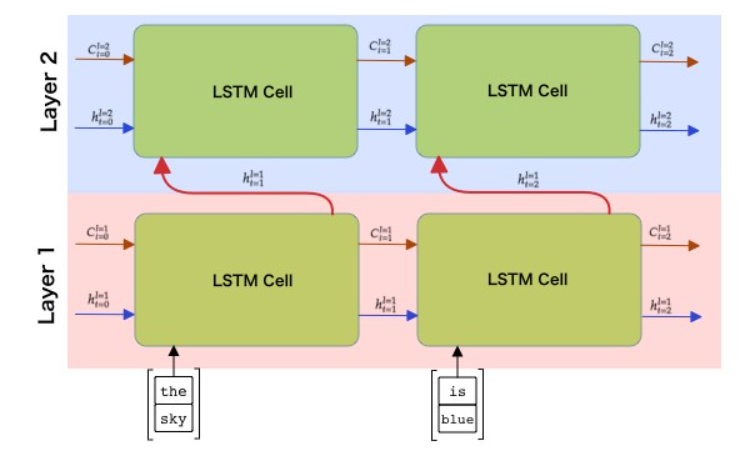
\includegraphics[width=10cm]{LSTM_MULTI.png}\caption{LSTM - Multi layer cells}\end{figure}
\subsubsection{LSTM - in context of rainfall}

\begin{itemize}
	\item 2018
	\begin{itemize}
		\item CAMELS - Data set
		\item 2-Layer LSTM -cells
		\item Input feature size $d=5$ - prcp(mm/day), srad(W/m2), tmax(C), tmin(C), vp(Pa). 
		\item Hidden state  size $h=20$
		\item Dropout rate = $10\%$
		\item Sequemce length - $365$ days. 
	\end{itemize} 
	\item 2019
	\begin{itemize}
		\item CAMELS - Data set
		\item 1-Layer LSTM 
        \item Input feature size $d=5$ ? 
		\item Hidden state  size $h=256$
		\item Dropout rate = $40\%$
		\item Sequemce length - $270$ days. 
	\end{itemize} 	
\end{itemize}

\newpage

\section{Results}

\subsection{Training results}

\subsection{Interpetabilty results}



\newpage
\section{References}

\begin{enumerate}
	\item \url{https://en.wikipedia.org/wiki/Long_short-term_memory}
	\item \url{https://machinelearningmastery.com/rectified-linear-activation-function-for-deep-learning-neural-networks}
	\item \url{	https://calvinfeng.gitbook.io/machine-learning-notebook/supervised-learning/recurrent-neural-network/recurrent_neural_networks}
	\item \url{https://calvinfeng.gitbook.io/machine-learning-notebook/supervised-learning/recurrent-neural-network/long_short_term_memory}
	\item \url{https://towardsdatascience.com/from-a-lstm-cell-to-a-multilayer-lstm-network-with-pytorch-2899eb5696f3}
	\item DigitalSreeni's Youtube channel - \url{https://www.youtube.com/watch?v=Mdp5pAKNNW4&t=238s}
	\item MIT lecture - Recurrent Neural Network - \url{https://www.youtube.com/watch?v=qjrad0V0uJE&t=3051s}
\end{enumerate}



$S_{b_1} = \big\{X_i, Y_i\big\}_{i=1}^{i=n_1}\quad , X_i,Y_i \sim f(X,Y| b_1) $  \\ \\
$S_{b_2} = \big\{X_i, Y_i\big\}_{i=1}^{i=n_2}\quad , X_i,Y_i \sim f(X,Y| b_2) $ \\

$S_{b_1} \cup S_{b_2}$ \\

$X$ \\ $Y$ \\ $ \big\{b_1, b_2\big\}$ \\ \\ 

$\text{Trained Model} \mapsto \text{Interpetabilty attributes}$ \\
$attributes_{\{S_{b_1} \cup S_{b_2}\}}$

	
\newpage




\nocite{*}
\printbibliography



\end{document}
